

\tikzset{every picture/.style={line width=0.75pt}} %set default line width to 0.75pt        

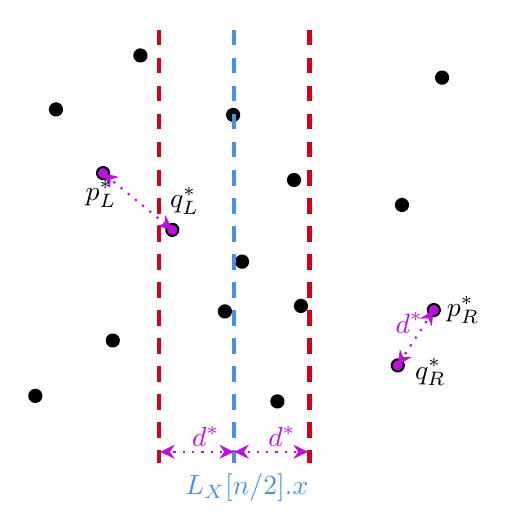
\begin{tikzpicture}[x=0.5pt,y=0.5pt,yscale=-1,xscale=1]
%uncomment if require: \path (0,347); %set diagram left start at 0, and has height of 347

%Flowchart: Connector [id:dp3585002987789013] 
\draw  [fill={rgb, 255:red, 0; green, 0; blue, 0 }  ,fill opacity=1 ] (229.06,171.88) .. controls (226.68,172.34) and (224.39,170.78) .. (223.94,168.41) .. controls (223.49,166.03) and (225.04,163.74) .. (227.42,163.29) .. controls (229.79,162.83) and (232.08,164.39) .. (232.54,166.77) .. controls (232.99,169.14) and (231.43,171.43) .. (229.06,171.88) -- cycle ;
%Flowchart: Connector [id:dp7980412079509043] 
\draw  [fill={rgb, 255:red, 0; green, 0; blue, 0 }  ,fill opacity=1 ] (94.58,61.88) .. controls (92.2,62.34) and (89.91,60.78) .. (89.46,58.41) .. controls (89,56.03) and (90.56,53.74) .. (92.94,53.29) .. controls (95.31,52.83) and (97.6,54.39) .. (98.05,56.77) .. controls (98.51,59.14) and (96.95,61.43) .. (94.58,61.88) -- cycle ;
%Flowchart: Connector [id:dp9736868983859984] 
\draw  [fill={rgb, 255:red, 0; green, 0; blue, 0 }  ,fill opacity=1 ] (155.62,22.88) .. controls (153.25,23.34) and (150.95,21.78) .. (150.5,19.41) .. controls (150.05,17.03) and (151.6,14.74) .. (153.98,14.29) .. controls (156.35,13.83) and (158.64,15.39) .. (159.1,17.77) .. controls (159.55,20.14) and (157.99,22.43) .. (155.62,22.88) -- cycle ;
%Flowchart: Connector [id:dp957649299032159] 
\draw  [fill={rgb, 255:red, 0; green, 0; blue, 0 }  ,fill opacity=1 ] (266.64,112.88) .. controls (264.27,113.34) and (261.98,111.78) .. (261.52,109.41) .. controls (261.07,107.03) and (262.63,104.74) .. (265,104.29) .. controls (267.37,103.83) and (269.67,105.39) .. (270.12,107.77) .. controls (270.57,110.14) and (269.02,112.43) .. (266.64,112.88) -- cycle ;
%Flowchart: Connector [id:dp9650319562783608] 
\draw  [fill={rgb, 255:red, 0; green, 0; blue, 0 }  ,fill opacity=1 ] (373.64,38.88) .. controls (371.27,39.34) and (368.98,37.78) .. (368.52,35.41) .. controls (368.07,33.03) and (369.63,30.74) .. (372,30.29) .. controls (374.37,29.83) and (376.67,31.39) .. (377.12,33.77) .. controls (377.57,36.14) and (376.02,38.43) .. (373.64,38.88) -- cycle ;
%Flowchart: Connector [id:dp1191629503329028] 
\draw  [color={rgb, 255:red, 0; green, 0; blue, 0 }  ,draw opacity=1 ][fill={rgb, 255:red, 189; green, 16; blue, 224 }  ,fill opacity=1 ] (178.64,148.88) .. controls (176.27,149.34) and (173.98,147.78) .. (173.52,145.41) .. controls (173.07,143.03) and (174.63,140.74) .. (177,140.29) .. controls (179.37,139.83) and (181.67,141.39) .. (182.12,143.77) .. controls (182.57,146.14) and (181.02,148.43) .. (178.64,148.88) -- cycle ;
%Flowchart: Connector [id:dp46368149090735455] 
\draw  [fill={rgb, 255:red, 189; green, 16; blue, 224 }  ,fill opacity=1 ] (341.62,246.88) .. controls (339.25,247.34) and (336.95,245.78) .. (336.5,243.41) .. controls (336.05,241.03) and (337.6,238.74) .. (339.98,238.29) .. controls (342.35,237.83) and (344.64,239.39) .. (345.1,241.77) .. controls (345.55,244.14) and (343.99,246.43) .. (341.62,246.88) -- cycle ;
%Flowchart: Connector [id:dp6008165035231083] 
\draw  [fill={rgb, 255:red, 0; green, 0; blue, 0 }  ,fill opacity=1 ] (216.64,207.88) .. controls (214.27,208.34) and (211.98,206.78) .. (211.52,204.41) .. controls (211.07,202.03) and (212.63,199.74) .. (215,199.29) .. controls (217.37,198.83) and (219.67,200.39) .. (220.12,202.77) .. controls (220.57,205.14) and (219.02,207.43) .. (216.64,207.88) -- cycle ;
%Flowchart: Connector [id:dp7362164431483738] 
\draw  [fill={rgb, 255:red, 0; green, 0; blue, 0 }  ,fill opacity=1 ] (222.64,65.84) .. controls (220.27,66.29) and (217.98,64.73) .. (217.52,62.36) .. controls (217.07,59.99) and (218.63,57.69) .. (221,57.24) .. controls (223.37,56.79) and (225.67,58.34) .. (226.12,60.72) .. controls (226.57,63.09) and (225.02,65.38) .. (222.64,65.84) -- cycle ;
%Straight Lines [id:da6529740224708328] 
\draw [color={rgb, 255:red, 74; green, 144; blue, 226 }  ,draw opacity=1 ][line width=1.5]  [dash pattern={on 5.63pt off 4.5pt}]  (222.5,0) -- (222.5,313) ;
%Flowchart: Connector [id:dp2239447293014194] 
\draw  [fill={rgb, 255:red, 0; green, 0; blue, 0 }  ,fill opacity=1 ] (135.64,228.88) .. controls (133.27,229.34) and (130.98,227.78) .. (130.52,225.41) .. controls (130.07,223.03) and (131.63,220.74) .. (134,220.29) .. controls (136.37,219.83) and (138.67,221.39) .. (139.12,223.77) .. controls (139.57,226.14) and (138.02,228.43) .. (135.64,228.88) -- cycle ;
%Flowchart: Connector [id:dp4443697198815304] 
\draw  [fill={rgb, 255:red, 0; green, 0; blue, 0 }  ,fill opacity=1 ] (254.64,272.88) .. controls (252.27,273.34) and (249.98,271.78) .. (249.52,269.41) .. controls (249.07,267.03) and (250.63,264.74) .. (253,264.29) .. controls (255.37,263.83) and (257.67,265.39) .. (258.12,267.77) .. controls (258.57,270.14) and (257.02,272.43) .. (254.64,272.88) -- cycle ;
%Flowchart: Connector [id:dp25292770923986996] 
\draw  [fill={rgb, 255:red, 189; green, 16; blue, 224 }  ,fill opacity=1 ] (128.64,107.88) .. controls (126.27,108.34) and (123.98,106.78) .. (123.52,104.41) .. controls (123.07,102.03) and (124.63,99.74) .. (127,99.29) .. controls (129.37,98.83) and (131.67,100.39) .. (132.12,102.77) .. controls (132.57,105.14) and (131.02,107.43) .. (128.64,107.88) -- cycle ;
%Flowchart: Connector [id:dp32241515903160844] 
\draw  [fill={rgb, 255:red, 0; green, 0; blue, 0 }  ,fill opacity=1 ] (79.64,268.88) .. controls (77.27,269.34) and (74.98,267.78) .. (74.52,265.41) .. controls (74.07,263.03) and (75.63,260.74) .. (78,260.29) .. controls (80.37,259.83) and (82.67,261.39) .. (83.12,263.77) .. controls (83.57,266.14) and (82.02,268.43) .. (79.64,268.88) -- cycle ;
%Flowchart: Connector [id:dp5412978107709706] 
\draw  [fill={rgb, 255:red, 0; green, 0; blue, 0 }  ,fill opacity=1 ] (344.64,130.88) .. controls (342.27,131.34) and (339.98,129.78) .. (339.52,127.41) .. controls (339.07,125.03) and (340.63,122.74) .. (343,122.29) .. controls (345.37,121.83) and (347.67,123.39) .. (348.12,125.77) .. controls (348.57,128.14) and (347.02,130.43) .. (344.64,130.88) -- cycle ;
%Flowchart: Connector [id:dp8188453538986455] 
\draw  [fill={rgb, 255:red, 189; green, 16; blue, 224 }  ,fill opacity=1 ] (367.64,206.88) .. controls (365.27,207.34) and (362.98,205.78) .. (362.52,203.41) .. controls (362.07,201.03) and (363.63,198.74) .. (366,198.29) .. controls (368.37,197.83) and (370.67,199.39) .. (371.12,201.77) .. controls (371.57,204.14) and (370.02,206.43) .. (367.64,206.88) -- cycle ;
%Straight Lines [id:da7981748798144619] 
\draw [color={rgb, 255:red, 189; green, 16; blue, 224 }  ,draw opacity=1 ] [dash pattern={on 0.84pt off 2.51pt}]  (130.14,105.49) -- (175.5,142.68) ;
\draw [shift={(177.82,144.59)}, rotate = 219.35] [fill={rgb, 255:red, 189; green, 16; blue, 224 }  ,fill opacity=1 ][line width=0.08]  [draw opacity=0] (10.72,-5.15) -- (0,0) -- (10.72,5.15) -- (7.12,0) -- cycle    ;
\draw [shift={(127.82,103.59)}, rotate = 39.35] [fill={rgb, 255:red, 189; green, 16; blue, 224 }  ,fill opacity=1 ][line width=0.08]  [draw opacity=0] (10.72,-5.15) -- (0,0) -- (10.72,5.15) -- (7.12,0) -- cycle    ;
%Straight Lines [id:da4570690123839587] 
\draw [color={rgb, 255:red, 189; green, 16; blue, 224 }  ,draw opacity=1 ] [dash pattern={on 0.84pt off 2.51pt}]  (342.44,240.07) -- (365.18,205.1) ;
\draw [shift={(366.82,202.59)}, rotate = 123.05] [fill={rgb, 255:red, 189; green, 16; blue, 224 }  ,fill opacity=1 ][line width=0.08]  [draw opacity=0] (10.72,-5.15) -- (0,0) -- (10.72,5.15) -- (7.12,0) -- cycle    ;
\draw [shift={(340.8,242.59)}, rotate = 303.05] [fill={rgb, 255:red, 189; green, 16; blue, 224 }  ,fill opacity=1 ][line width=0.08]  [draw opacity=0] (10.72,-5.15) -- (0,0) -- (10.72,5.15) -- (7.12,0) -- cycle    ;
%Straight Lines [id:da3441187372234148] 
\draw [color={rgb, 255:red, 208; green, 2; blue, 27 }  ,draw opacity=1 ][line width=1.5]  [dash pattern={on 5.63pt off 4.5pt}]  (168,0) -- (168,313) ;
%Straight Lines [id:da06503609524950982] 
\draw [color={rgb, 255:red, 208; green, 2; blue, 27 }  ,draw opacity=1 ][line width=1.5]  [dash pattern={on 5.63pt off 4.5pt}]  (277,0) -- (277,313) ;
%Straight Lines [id:da01899195473791948] 
\draw [color={rgb, 255:red, 189; green, 16; blue, 224 }  ,draw opacity=1 ] [dash pattern={on 0.84pt off 2.51pt}]  (172,305) -- (219.5,305) ;
\draw [shift={(222.5,305)}, rotate = 180] [fill={rgb, 255:red, 189; green, 16; blue, 224 }  ,fill opacity=1 ][line width=0.08]  [draw opacity=0] (10.72,-5.15) -- (0,0) -- (10.72,5.15) -- (7.12,0) -- cycle    ;
\draw [shift={(169,305)}, rotate = 0] [fill={rgb, 255:red, 189; green, 16; blue, 224 }  ,fill opacity=1 ][line width=0.08]  [draw opacity=0] (10.72,-5.15) -- (0,0) -- (10.72,5.15) -- (7.12,0) -- cycle    ;
%Straight Lines [id:da5930514326113744] 
\draw [color={rgb, 255:red, 189; green, 16; blue, 224 }  ,draw opacity=1 ] [dash pattern={on 0.84pt off 2.51pt}]  (225.5,305) -- (273,305) ;
\draw [shift={(276,305)}, rotate = 180] [fill={rgb, 255:red, 189; green, 16; blue, 224 }  ,fill opacity=1 ][line width=0.08]  [draw opacity=0] (10.72,-5.15) -- (0,0) -- (10.72,5.15) -- (7.12,0) -- cycle    ;
\draw [shift={(222.5,305)}, rotate = 0] [fill={rgb, 255:red, 189; green, 16; blue, 224 }  ,fill opacity=1 ][line width=0.08]  [draw opacity=0] (10.72,-5.15) -- (0,0) -- (10.72,5.15) -- (7.12,0) -- cycle    ;
%Flowchart: Connector [id:dp173337509020409] 
\draw  [fill={rgb, 255:red, 0; green, 0; blue, 0 }  ,fill opacity=1 ] (271.64,203.88) .. controls (269.27,204.34) and (266.98,202.78) .. (266.52,200.41) .. controls (266.07,198.03) and (267.63,195.74) .. (270,195.29) .. controls (272.37,194.83) and (274.67,196.39) .. (275.12,198.77) .. controls (275.57,201.14) and (274.02,203.43) .. (271.64,203.88) -- cycle ;

% Text Node
\draw (185,318.45) node [anchor=north west][inner sep=0.75pt]  [color={rgb, 255:red, 74; green, 144; blue, 226 }  ,opacity=1 ] [align=left] {$\displaystyle L_{X}[ n/2] .x$};
% Text Node
\draw (113,106.45) node [anchor=north west][inner sep=0.75pt]   [align=left] {$\displaystyle p_{L}^{*}$};
% Text Node
\draw (174,111.45) node [anchor=north west][inner sep=0.75pt]   [align=left] {$\displaystyle q_{L}^{*}$};
% Text Node
\draw (374,190.45) node [anchor=north west][inner sep=0.75pt]   [align=left] {$\displaystyle p_{R}^{*}$};
% Text Node
\draw (351,235.45) node [anchor=north west][inner sep=0.75pt]   [align=left] {$\displaystyle q_{R}^{*}$};
% Text Node
\draw (337,202.41) node [anchor=north west][inner sep=0.75pt]  [color={rgb, 255:red, 189; green, 16; blue, 224 }  ,opacity=1 ] [align=left] {$\displaystyle d^{*}$};
% Text Node
\draw (190,284.41) node [anchor=north west][inner sep=0.75pt]  [color={rgb, 255:red, 189; green, 16; blue, 224 }  ,opacity=1 ] [align=left] {$\displaystyle d^{*}$};
% Text Node
\draw (245,284.41) node [anchor=north west][inner sep=0.75pt]  [color={rgb, 255:red, 189; green, 16; blue, 224 }  ,opacity=1 ] [align=left] {$\displaystyle d^{*}$};


\end{tikzpicture}

